\section{Introduction}

\begin{frame}\frametitle{\secname}\framesubtitle{Project Introduction}
\begin{columns}[c,totalwidth=\textwidth]
    \column{0.56\textwidth}
    \begin{itemize}
        \item <1-> VolumetricSynth is a JUCE-based plugin for real-time 3D timbre blending.
        \item <2-> It extends classic 2D vector synthesis to an 8-corner 3D interpolation model.
        \item <3-> Goal: improve expressive sound design while keeping control intuitive.
        \item <4-> This presentation: goals, ownership, progress, remaining work, and timeline to May 5.
    \end{itemize}

    \column{0.44\textwidth}
    \centering
    \vfill
    {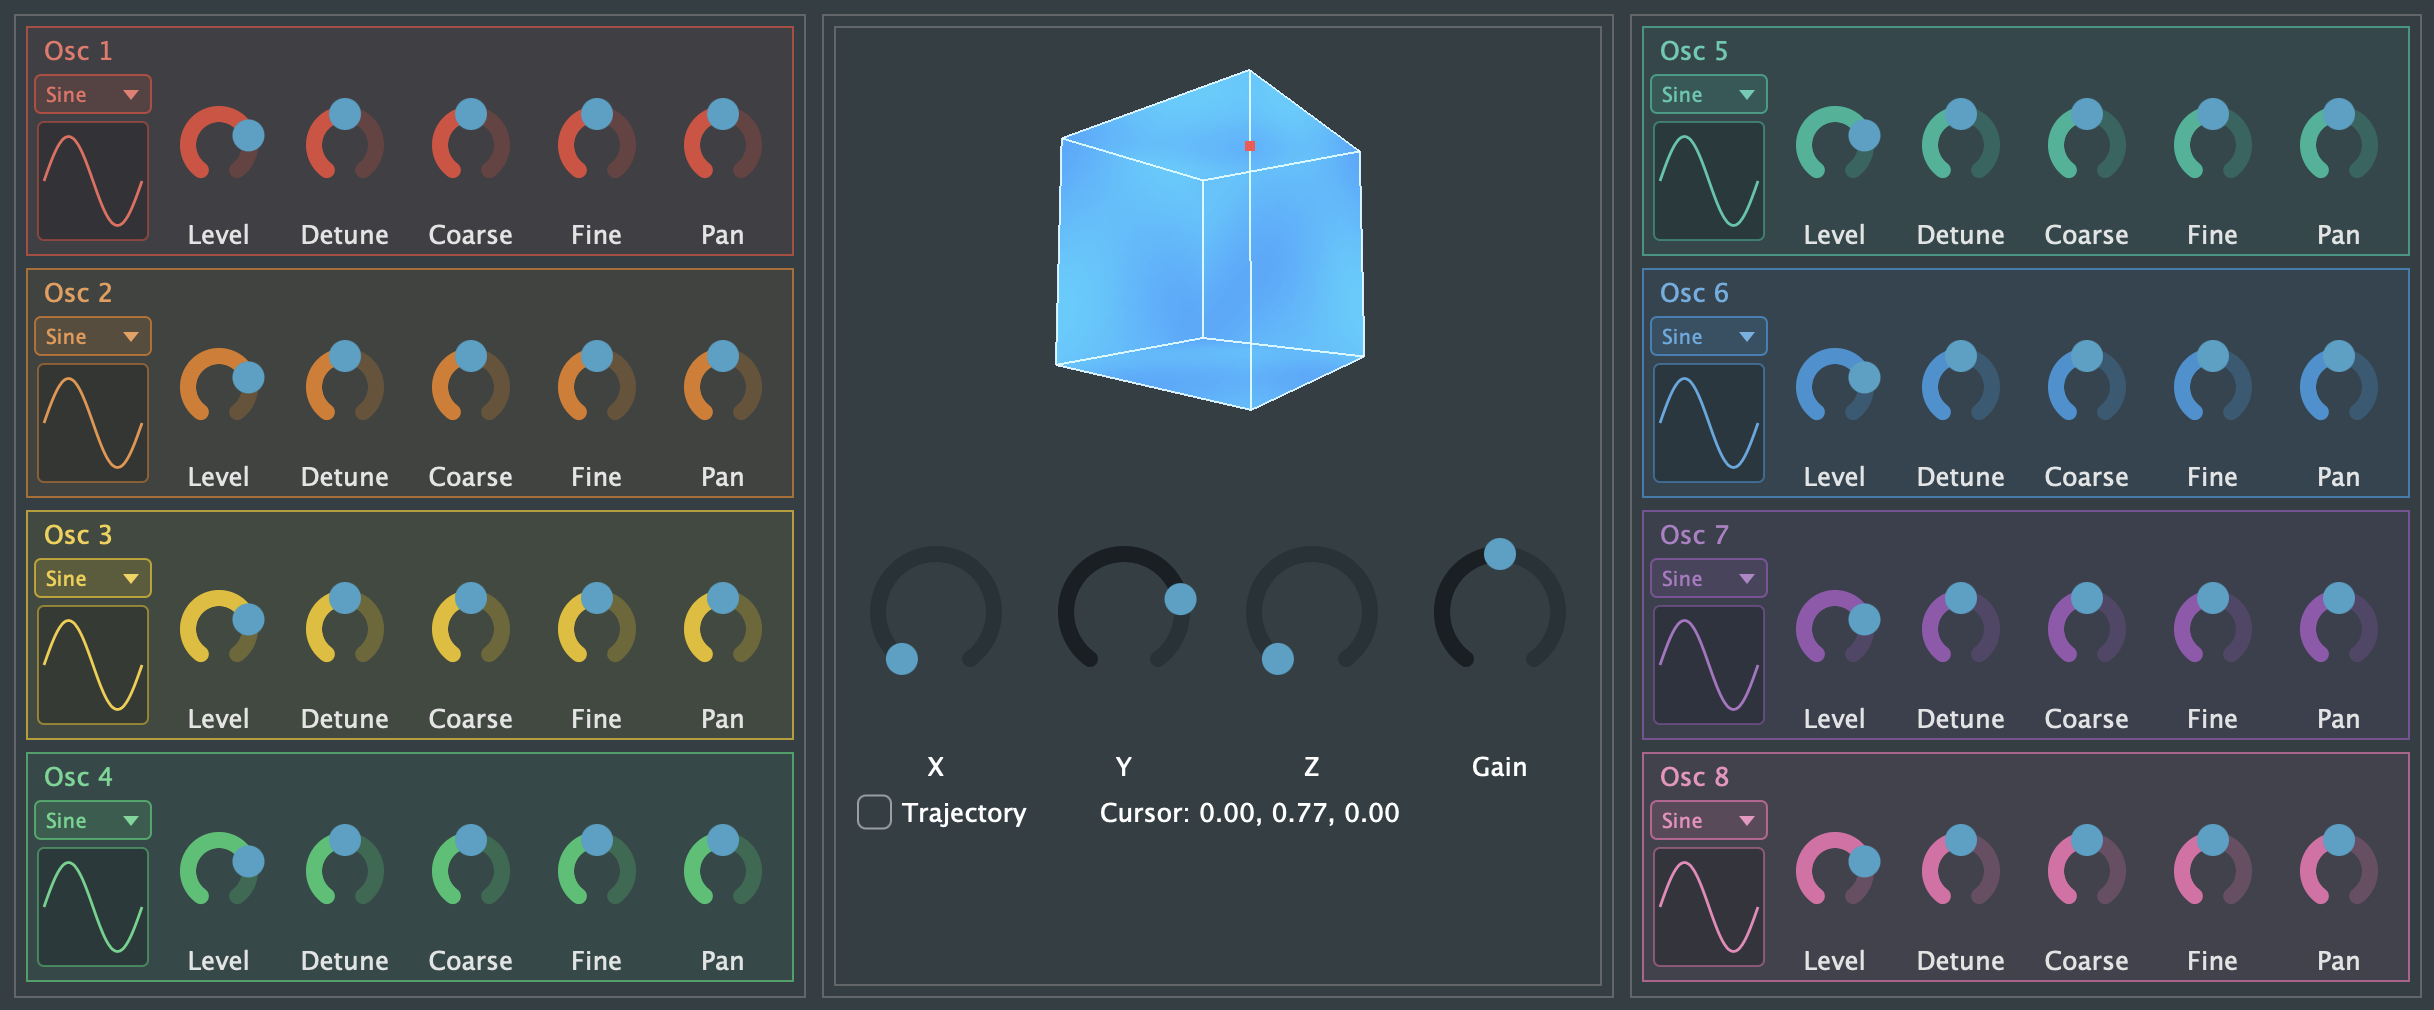
\includegraphics[width=\linewidth,height=0.72\textheight,keepaspectratio]{figures/pluginss.png}}

    \vfill
\end{columns}
\end{frame}
